\section{Examples from iOS development using Swift}\label{sec:03}

In previous chapter we described the problematic of MVC approach in Apple`s example. So there is a question: «How to use proper layered architecture in an iOS app, what its advantages and disadvantages will be?». The community came with an idea of using MVVM architecture aka proper MVC. Model-View-ViewModel is a response for inappropriate MVC, which came as a resue because of impossibility to test business logic of an application. So the main point is to separate any UI with business logic. We have a dummy view in UIViewController aka UI layer aka View, business logic in ViewModel aka Domain layer and Networking/Persistence/Other managers in Model aka Infrastructure layer. Still we are missing Application layer, so this responsibility might be taken by UIViewController, but we do not want this for sure and Coordinator pattern comes to rescue. Coordinator pattern separates UI layer from Application layer. In the end we have such modules connection.
\begin{figure}[!htbp]
	\centering
	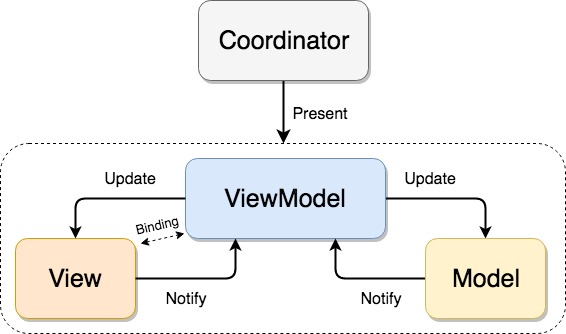
\includegraphics[width=0.95\linewidth]{sections/02-chapter/images/Coordinator.jpg}
	\caption{MVVM-C architecture.}\label{sec:02_01:fig:02}
	\end{figure}
    
Imagine that you are simply separating those concerns you can not only copy-paste Domain layer, Application layer and Model layer code from iOS to MacOS/WatchOS/tvOS app(only rewriting UI layer) but also Unit-tests which you used to cover you ViewModel. Bingo!!! Everything looks super-great, well in theory it is. But in practice we stuck in some serious issues, mostly related to data binding. What is data binding? Well, imagine that you have a two classes which are connected via composition. In our example it is UIViewController has a property called ViewModel. How to make UI respond to changes in ViewModel? How to make ViewModel react to changes in persistence storage? How to make ViewModel react to changes on server(let`s imagine we have a hook)? How to make UI react to changes in database? So communication between so many layers becomes a serious issue. We have a lot of solutions: callback via closures aka lambda function, delegates, some reactive binding etc. While MacOS sdk provides native data binding called Cocoa-bindings we do not have any useful instrument in iOS SDK and have to use callback, specifying that it have to be called on main thread each time etc. But community comes to rescue ti Rx frameworks (RxSwift and RxCococoa) and huge amount of useful reactive extensions. Those frameworks are universal for all Apple platforms, which makes them very useful and extremilly popular. Everything looks super-great but for one thing. Reactive programming is another  galaxy in development, which is so far from Junior developers that you should forget the idea of making cool reactive app with team who has those guys in it. Those frameworks requires changing a mindset from object-oriented programming to reactive functional programming which is not so easy. We can not use any reactive framework for sure and simply live with native solutions which we have from the box - callbacks and delegates, those patterns much easier to understand and use but they requires a lot of code, which slows down the development process and sometimes becomes very confusing to have dozens of objects which a delegates to other dozens of objects. I guess a team-leader should pick the most suitable solution for the particular team and particular project needs. Maybe MVC-C will become a great solution in terms of complexity/speed, maybe MVVM-C with delegates is a good one or even classic MVC is enough for project with no possibility of user action(for ex. currency exchange app which only provides info).
